\section{Singapore Electronic Road Pricing (ERP)}\label{sec:erp}

\subsection{Implementation}

Over time, ALS became hard to administer as Singaporean authorities priced vehicles more precisely. \citet[p. 4]{Chin2009} describes ALS once multiple charging periods and vehicle classes had been added: ``There were 16 different types of licences in use at its peak, and much concentration by the enforcement officers was required to ensure that they identified them correctly.'' The license system also precluded charging for each entry or varying prices much by time-of-day.

Therefore, in 1990 Singapore solicited bids for a wireless system which would be called, like Hong Kong's, Electronic Road Pricing (ERP). Wary of the privacy concerns that had bedeviled Hong Kong, authorities chose a ``smart card'' system: a roadside beacon tells a device on the vehicle to deduct money from a stored-value card, so that records of vehicle movements need not be kept \citep[p. 5]{Chin2009}. In 1995, the contract for the system was awarded to a consortium led by Phillips Singapore, and after extensive field trials, publicity and a limited implementation, ERP commenced full operation for private vehicles on September 1st, 1998. Tolls for commercial vehicles and taxis were phased in over the next three years, as these vehicles cross many tolling sites per day \citep[p. 64]{Menon2004}.

\subsection{Design}

ERP is precisely designed, with tolls that vary over times and vehicle types as well as a complex geography. Figure \ref{fig:singapore-toll-schedule} illustrates a weekday toll schedule to enter the primary CBD cordon in different years. For the first five years of ERP, tolls changed only at half-hour intervals, but since February 2003, whenever tolls change by more than S\$1, there is a five-minute interval in which tolls rise or fall by half the amount of the change, in order to discourage cars from slowing down or speeding up when tolls are about to change \citep{Menon2004}. Tolls in the CBD are only charged to inbound traffic. 

Technologically, \citet{Menon2004} describes ERP as having three components:

\begin{itemize}
\item In-vehicle Unit (IU), an electronic device that sits on vehicles' dashboards or handlebars. The IU has a slot for a ``CashCard'' that the user can load up with money at various establishments---similar to transit touch cards in wide use today. There are IU's for each of six vehicle classes (see Figure \ref{fig:singapore-IUs}), because the toll charged to a vehicle is a multiple of its ``Passenger Car Unit'' (PCU), an index of size (see Table \ref{tab:passenger-car-units}). Since 2008, instead of using the CashCard drivers use various services to have their credit cards charged \citep{Chew2009}.

\item Gantries, metal archways positioned in pairs over the road at tolling sites. When a vehicle passes below, the first gantry tells the vehicle's IU to charge appropriately. An optical sensor on the second gantry confirms the vehicle type matches the IU. In the event of a transaction error, a camera on the first gantry captures the rear number plate. 

\item The central control system, which verifies charges and issues notices and fines when there is a violation or error.
\end{itemize}

\begin{table}
	\begin{tabular}{|c|c|}
		\hline 
		PCU's & Vehicles\tabularnewline                              
		\hline 
		\hline 
		0.5   & motorcycles\tabularnewline                           
		\hline 
		1     & cars, taxis, light goods vehicles\tabularnewline     
		\hline 
		1.5   & heavy goods vehicles/small buses\tabularnewline      
		\hline 
		2     & very heavy goods vehicles/large buses\tabularnewline 
		\hline 
	\end{tabular}
	
	\caption{
	Passenger Car Units (PCU's) for ERP. Vehicle charges are weighted by the PCU number---e.g., a very heavy goods vehicle pays four times what a motorcycle does. \citep{LTA2016} 
	}
	\label{tab:passenger-car-units}
\end{table}

	
\begin{figure}
	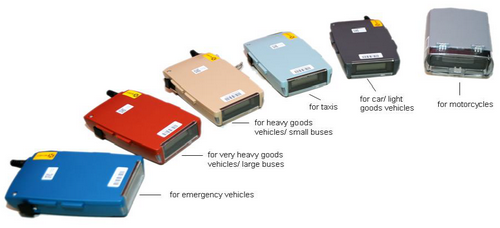
\includegraphics[width=4in]{../img/singapore-IUs.jpg}
	\caption{ERP In-vehicle units. https://www.lta.gov.sg/content/ltaweb/en/roads-and-motoring/managing-traffic-and-congestion/in-vehicle-unit-iu.html}
	\label{fig:singapore-IUs}
\end{figure}

\begin{figure}
	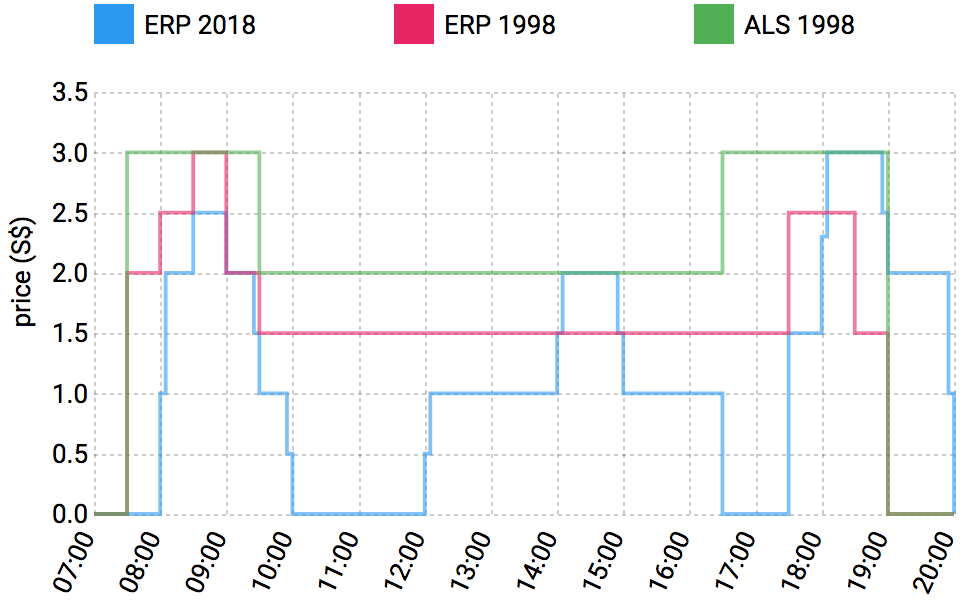
\includegraphics[width=1\textwidth]{../img/singapore-prices.png}
	\caption{Singapore prices for different years. The schedule becomes more variable as years pass. Note that the ALS price is not exactly comparable, as it permitted unlimited entries.}
	\label{fig:singapore-toll-schedule}
\end{figure}

The substantial changes to ERP have been spatial. ERP started in 1998 with 28 tolling sites replacing the extant ALS tolling sites and five on expressways \citep{Menon2010}. Since then, the scheme has been greatly expanded. Today, 39 tolling sites enclose three contiguous sub-cordons in the CBD. One, the Orchard Road Cordon, contains shopping areas and is thus unpriced on weekday mornings. The other two---the Bugis-Marina Centre Cordon and the Shenton Way-Chinatown Cordon---contain offices and thus operate all day during the weekdays. In the morning, traveling between these two sub-cordons is free---effectively making a single CBD cordon---but there is a small charge to do so between 6 and 8 PM, in order to limit intra-CBD congestion. There are also 54 tolling sites further out from the CBD to control traffic on expressways and particular roads.

The Land Transport Authority (LTA) updates tolls to target speeds of 20-30 kph on downtown roads and 45-65 kph on expressways \citep[pp. 6-7]{Menon2010}. They do so in the following way: Every three months the LTA checks speeds on the roads at different half-hours of the day. If, for some half-hour interval, the 85th percentile speed measured is above 65 kph on an expressway or 30 kph on downtown roads, the price is reduced for that half-hour; likewise, if the same measure is below 45 kph on an expressway or 20 kph on downtown roads, tolls rise. These are the speeds at which the LTA believe traffic flow is maximized \citet[p. 42]{Menon2000}. Speeds stabilized within a few years of charging, so not many price changes occur with each review \citet[p. 7]{Chin2009}.

\subsection{Transportation impacts}

The transition to ERP was not as thoroughly documented as the launch of ALS but some facts appear in reports written by LTA officials. Entries to the CBD fell by about 15\% per day and 16\% during the morning peak \citep[p. 42]{Menon2000}. However, only about 2\% of travelers cancelled their trips and there was no switch to public transit, which is unsurprising given that the charge to enter the CBD once was lower than under ALS. The reduction in entries is due partly to rerouting and retiming but mainly to a fall in repeat trips: since ALS permitted unlimited same-day entries, about 23\% of trips had been repeat trips---e.g., office workers using cars for lunches and meetings in the middle of the day \citep[p. 23]{Chin2009}. While there was initially increased congestion on a bypass route, presumably this has been corrected with the addition of tolling sites. 

There are no exemptions to ERP, so it cannot provide evidence of Theme I. Regarding Theme II, \citet{Olszewski2005} conclude, using data from before and after ERP, that the LTA's charging structure has done a good job controlling demand by spreading traffic over the day.

\subsection{Finances}

Implementation cost S\$197 million in 1998, of which S\$100 million paid for IU's (since the launch this expense is incurred by the vehicle owner) and S\$97 million to build out the infrastructure \citep{Santos2004}. Annual operating costs have measured about 20-30 percent of revenues \citep{Chin2009}.

ERP revenues in 1999 were S\$68 million---down a third from the S\$100 million earned by ALS and the Road Pricing Scheme in 1998 \cite[p. 34]{Goh2002}. Revenues fell because ERP prices were lower than the ALS charge, which, combined with the significant investment cost and higher operating cost, makes it clear that the switch to ERP was not motivated by revenue concerns. In 2012 ERP revenues were S\$159 million \citep{Chen2012}. Revenue is not hypothecated but rather flows into the governent's general fund.
